\chapter{The \FRAMEWORK}
\thispagestyle{plain}

\label{Framework}

% What does the framework do? It build meta-models that map between agent-level and system-level.
\framework builds meta-models that map the values of agent-level control parameters and system-level properties, and vice versa.
Learning both of these mappings are separate problems, which I call the \textit{forward-mapping problem} and the \textit{reverse mapping problem}.
To solve these problems, a user of \fw ``plugs in" a regression algorithm of their choice.
The framework uses this regression algorithm to learn the mappings and provide a user with an interface to query them.
Once the mappings are learned, the user can query either for \textit{prediction} or \textit{control}.
A prediction query asks the forward mapping to give a value for system-lev
Most of the implementation details and inner workings of \fw are abstracted away from the user, who only has to attend to a limited number of configuration points.

In this chapter, I will discuss the design goals of \fw, the framework structure, software implementation details, and how well \fw conforms to the design goals.

% It frames the mapping problem into the forward mapping and the reverse mapping
% Uses a pluggable regression algorithm to solve these mapping problems

\section{Design Goals of The \framework}

% Our specific goals: provide insight and more intuitive control to agent-based models with a approach that is domain independent, algorithm independent, accurate and fast for the user.
My specific goal in designing \fw is to make controlling and interacting with agent-based models more intuitive.
In addition to this central goal, \fw strives to be:
\begin{itemize}
  \item Domain independent -- the design of \fw should minimize the amount of configuration for each domain,
  \item Algorithm independent -- any regression algorithm should be able to be plugged into \fw,
  \item Accurate -- \fw should generate accurate predictions and control suggestions,
  \item Fast for the user -- interactions with the models generated by \fw should require minimal computational time.
\end{itemize}

% Domain independence is important because the variety in which ABMs come. We want the same general approach to work for a forest fire simulation, a boid flock or particle swarm optimization.
% Algorithm independence is important because different algorithms will model different domains better. Also, as new regression techniques are implemented in the future, they can be plugged in to increase the accuracy of \fw.
Domain independence is paramount because of the variety in which ABMs come.
I have designed \fw such that the same general approach would work for any ABM.
Also, I strove to minimize the amount of configuration needed to apply \fw to a new domain.
These constraints I have set on the design make \fw broadly applicable to a number of domains, without the need of in-depth domain knowledge.
To reinforce this claim, I have tested \fw on a number of diverse domains and used the same general approach for each.

Algorithm independence in a learning framework is important because different algorithms are more effective for modeling different agent-based models.
In general, the learning algorithms that will be discussed in this dissertation will satisfy the requirements for modeling most agent-based models.
However, an in depth analysis of which types of algorithms should be used for different classes of ABMs is outside the scope of this dissertation research.
In addition, algorithm independence allows \fw to scale with new advances in machine learning research, since future state-of the art regression algorithms can be plugged in just as easily as current approaches.

Accuracy and fast user response time appear to be obvious design goals.
However, \fw requires that the user spends a significant amount of computational time sampling different configurations of the target ABM.
These large training sets can be used to build static meta-models of ABMs that are both accurate and fast to query.
In contrast, an active learning approach would be able to learn models faster, but would require interaction with the user, increasing the amount of user interaction.
Likewise, optimization approaches could be used to generate arbitrarily accurate results, but typically require numerous iterations and would significantly increase the response time for a user's query.
In summary, I am making the assumption that users studying ABMs with \fw are more interested in achieving more accurate results for their research, than generating their results faster.






\section{Framework Structure}

% The framework is split into three phases and four major parts.
The framework is split into several phases: sampling, solving the forward mapping problem, solving the reverse mapping problem, querying for prediction, and querying for control (i.e., suggesting a configuration).
This section uses the diagram in Figure \ref{fig:frameworkdiag} to explain how the different phases interact with one another.
From an exterior perspective, the framework only has a limited about of input and output:
\fw takes in observations of an agent-based model and then provides interfaces to query for prediction and control.
These queries interact with the user, as well as the agent-based model.

Many configuration points exist, which allow users of \fw to modify the behavior of the framework.
However, the individual phases take the same output and provide the same output, no matter the configuration.
This is what makes \fw a framework and not a collection of algorithms.
For example, even though different regression algorithms can be used to learn the forward mapping, the forward mapping still provides predictions of how an ABM will behave, from the user's perspective.

% Each phase feeds into the next
% Many configuration points exist in which users of \fw can change the way the framework works.
% However, no matter the configuration, the input and output of each phase is the same.

% Diagram  sampling ->  [ FM / RM ] -> usage tools





%% HACK!! I need to physically move this around
\begin{figure}[H]
\centering
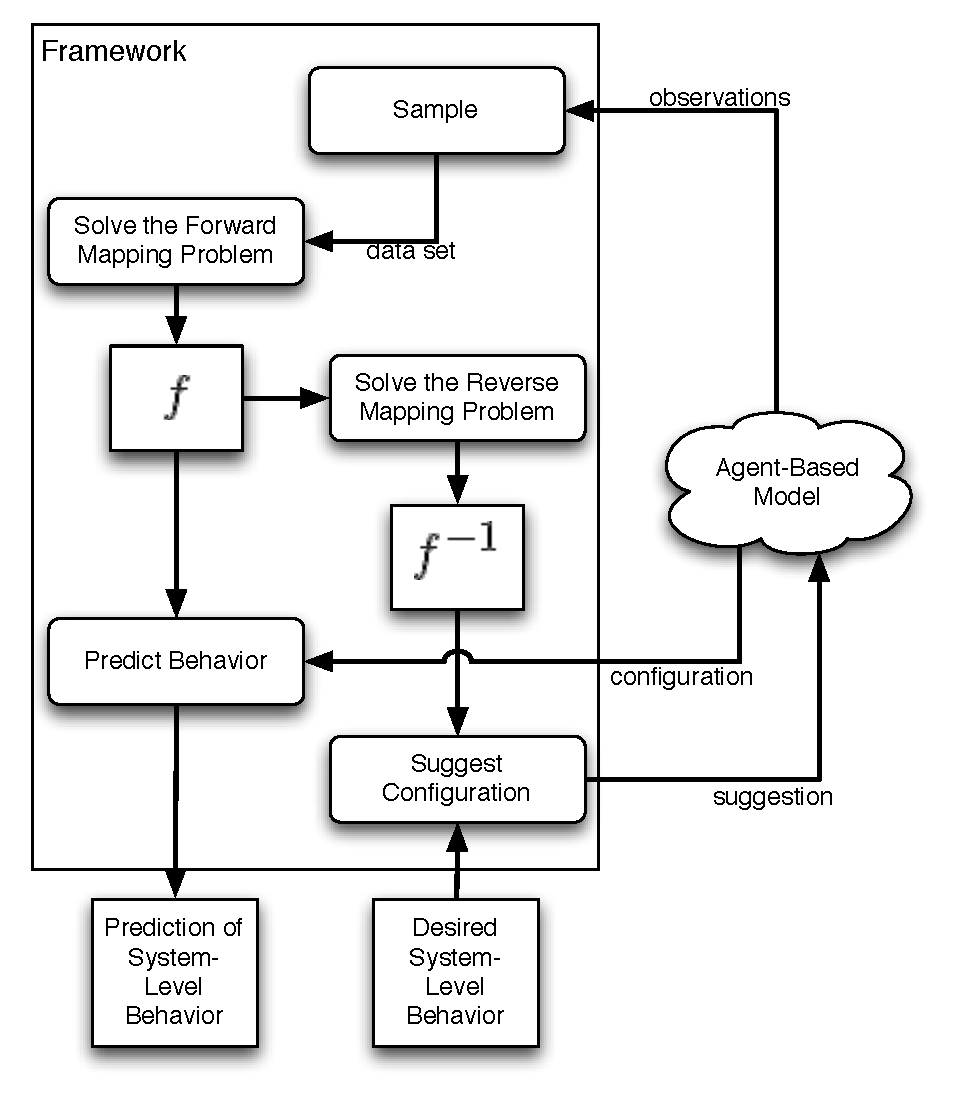
\includegraphics[scale=1]{images/framework.pdf}
\caption{An overview of the phases of \fw and how data flows between them.}
\label{fig:frameworkdiag}
\end{figure}

\subsection{Defining System-Level Behavior Properties}
   % Measurements have to be defined to tell what to sample.
System-level properties of an ABM must be defined by the user of \fw.
The measurement is some sort of statistical or mathematical calculation based on the state of the ABM over some period of time.
   % Measurements must be stable (i.e., follow the laws of large numbers); they must converge over time
The one assumption made by \fw is that the measurement is \textit{stable}, meaning that as the same configuration is sampled again and again, the measurement's value should vary very much.
One way to measure stability is to calculate the standard deviation of measured values of several runs of the system.
   % Wording of the measurement is important (give the example of wolves going extinct)
The need for this assumption, ways to conform to it and a more detailed explanation of how to define system-level properties is provided in Chapter \ref{Defining}: Defining System-Level Behaviors.


\subsection{Sampling}
% The first phase is sampling, in which the framework interacts with the agent-based model to generate a large enough data set for training.
The first phase is \textit{sampling}.
In this phase, numerous observations are made on different configurations of an agent-based model.
A data set is generated that contains the independent variables (the agent-level control parameter values) and the resultant system-level behaviors that are measured.
This process can be significantly time consuming, dependent on several factors:
\begin{itemize}
  \item Execution time of the model -- the models will be executed numerous times, so the longer a model takes to execute, the longer the whole set of experiments will take to execute,
  \item Granularity -- more detailed samplings will take more time, since more points must be sampled,
  \item Dimensionality -- more agent-level control parameters result in a larger search space and naturally more points to sample,
\end{itemize}
Small samples, such as 120 observation sample of the NetLogo \textit{Fires} model\footnote{See Chapter \ref{Results} for detailed results} \cite{fires} , required about thirty seconds.\footnote{Most experiments are executed on a 2.2GHz Intel Core 2 Duo running Mac OS X}
Meanwhile, a large sample of 50000 observation of a Reynolds boid flock \cite{reynolds1987} took approximately four days.

The user is required to have a minimal amount of domain knowledge to specify to \fw what ranges of values should be sampled.
\fw is not able to automatically infer which value ranges are interesting, and thus must be explicitly defined.

One redeeming quality of this process is that it is easily parallelizable.
Since each experiment is independent on one another, the set of all experiments can be segmented among a number of systems and processors to significantly reduce the computation time.
Once each subset of experiments are done executing, the results can be concatenated into one data set.

   % For this dissertation, we either use a random sampling method or a systematic sampling method
   % Future work: plug in different advanced sampling methods
For the scope of this dissertation, I limit \fw to use a simple random sampling method (i.e., randomly select points within a specified range) or a systematic sampling method (i.e., given ranges, sample evenly spaced points).
I acknowledge that an intelligent sampling strategy can be improve the performance of many machine learning techniques, however, none are used for the sake of focusing on other portions of the framework.
In future work, different sampling techniques' effect on accuracy and speed could be measured.



\subsection{The Forward-Mapping Problem}

% The second phase is learning the forward and reverse mapping.
% This is the main focus of the learning framework.

% Explain the forward mapping problem; give an example [figure]
The forward-mapping problem is to develop a function $f: \mathbb{R}^n \rightarrow \mathbb{R}$ that maps a provided configuration vector $\mathbf x = \{x_1, x_2, ..., x_n \}$ to a single system-level behavior property $\hat y$:
\[\hat y \leftarrow f(\mathbf x)\]
The set of values $\vec x$ consists of all the agent-level parameters (independent variables) in the data set provided by the sample step.
An individual mapping is learned for each system-level behavior measurement provided by the user.
% The forward mapping is a straightforward regression problem ... Assuming this is a many-to-one relationship (due to the correct definition of the measurement)

This problem is solved with straightforward regression, such as k-nearest neighbor.
% A regression algorithm needs to be initialized with the data set (if necessary). For example, a linear regression approach would solve the least-squares problem to generate the model. Meanwhile, something like KNN has no initialization time.
In this phase of \fw, the regression algorithm is ``initialized," if necessary.
For example, linear regression would need to solve the least-squares problem.
Meanwhile, an algorithm like k-nearest neighbor would not need to initialize anything.
% The forward mapping problem returns an object that can be queried for configuration vector x, and returns system-level property y.
Once this phase is completed, the user is provided with $f$, an interface to the mapping built by the regression algorithm.

A more in depth definition of the forward-mapping problem, specific examples of regression methods used in \fw, and the role of regression is given in Chapter \ref{ForwardMapping}: The Forward-Mapping Problem.


\subsection{The Reverse-Mapping Problem}

% Explain the reverse mapping problem; give an example [figure]
The reverse-mapping problem is to \textit{invert} the forward mapping.
This will produce a mapping $ f^{-1}: \mathbb{R} \rightarrow \hat S$ from a given system-level behavior property $y$ to a set of
configurations $ \hat S = \{ \mathbf {\hat x} | f( \mathbf {\hat x}) = y \}$.
That is, $S$ is the set of behaviors that will produce behavior $y$.
% The reverse mapping is an "inverted" regression problem.

% We invert the forward mapping
% Inverted regression means f^-1 (building an inverted mapping)
Developing the mapping $f^{-1}$ is what I call ``inverted regression problem," and has several unique challenges.
The main challenge is $f^{-1}$ does not describe a functional mapping.
This is because $f^{-1}$ describes a one-to-many relationship, since $f$ is many-to-one.
Therefore, \fw cannot use standard regression techniques to solve this problem.
Instead, \fw approximates the inverse of the forward mapping, with a method that I developed.
As an aside, this approach has the benefit of using the forward mapping to develop the reverse mapping.
No additional input from the user or data set are needed.
The intricacies of inverting a functional mapping developed by a regression algorithm are discussed in Chapter \ref{ReverseMapping}: The Reverse-Mapping Problem.
% Elude that we will discuss our particular solutions to these problems in later chapters

\subsection{Using the Maps}

% Explain how the maps are queried.
% Querying the forward mapping (example)
% Querying the reverse mapping (example)

% Possible uses: prediction and control


\subsection{Summary of Configuration Points}
% Sampling methodology
% Measurements
% Forward Mapping Algorithm
% Reverse Mapping Algorithm

\section{Software Implementation Details}
% Most of the software is implemented in python, but the interaction with NetLogo is handled with Java, so that I can access the Java API.

% Give a list of agent-level variable ranges/steps
% Generate the experiments list
% Samples a NetLogo ABM with Java API, given the list of experiments, save the results
% Interact with the forward mapping regression algorithm with a python module interface
% Interact with the reverse mapping approach (discussed more in Chapter X) with a python module interface
% Different tools for selecting solutions and visualizing slices are separate python scripts.

% An overarching "master script" written in python that glues these together and automatically transitions from one to another. Each stage can be performed one by one

% More about NetLogo is covered in Background.


\section{Example: \fw Applied to Wolf Sheep Predation}

% Identification of agent-level control parameters
% Identify ranges of values for agent-level control parameters

% Definition of system-level measurements.
% Specifically how to measure them

% Choice of regression algorithm (KNN)  -- More discussion is on FM and RM

% Analysis of the accuracy of our approach against this domain is in the RESULTS chapter.

% Give a glimpse into tools -- More discussion is on using chapter


\section{Analysis of \fw  vs. the Design Goals}
% Our framework is domain independent, because it reduces the forward mapping problem to a classical regression problem of learning the correlation between the agent-level parameters and the system-level properties..
% We introduce a domain-independent approach to solve the reverse mapping problem that uses standard regression to build a space of configurations that would produce desired behavior.

% Our framework is algorithm independent, because any regression algorithm (e.g., ...) can be used to develop the forward mapping and the reverse mapping

% Our framework is as accurate as the regression algorithms used and the data set sampled from the agent-based model. /elaborate/
% In general, I prefer spending longer sampling to generate an exhaustive data set increase accuracy and reducing user interaction delays when querying for a prediction or a suggestion for controlling.
% This shifts most of the computation time offline, instead of online, reducing user interaction time when querying the forward or reverse mappings.
